\documentclass[tikz, border=1mm]{standalone}
\usepackage{tikz} 
\usetikzlibrary{arrows.meta}
\usepackage{pgfplots}

\begin{document}

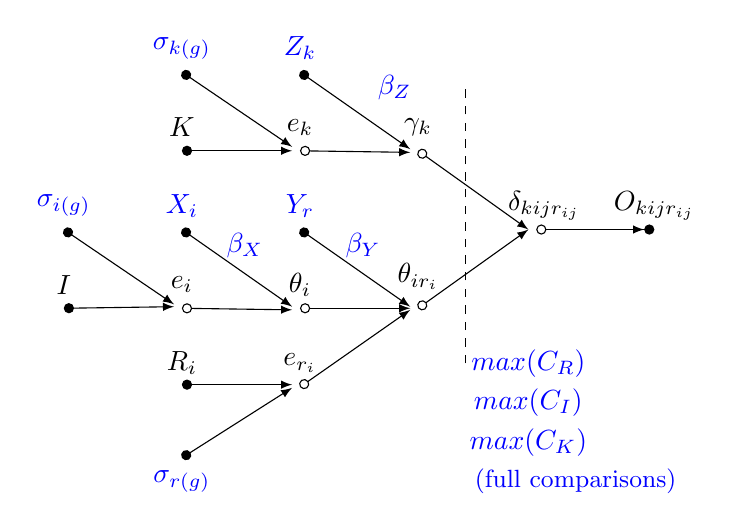
\begin{tikzpicture}

    % main graph
    % nodes (variables)
    \node at (-3,1) {\textcolor{blue}{$X_{i}$}};
    \node at (-3,0) {$e_{i}$};
    \node at (-1.5,3) {\textcolor{blue}{$Z_{k}$}};
    \node at (-1.5,2) {$e_{k}$};
    \node at (-1.5,1) {\textcolor{blue}{$Y_{r}$}};
    \node at (-1.5,0) {$\theta_{i}$};
    \node at (-1.5,-1) {$e_{r_{i}}$};
    \node at (0,2) {$\gamma_{k}$};
    \node at (0,0.1) {$\theta_{ir_{i}}$};
	\node at (1.6,1) {$\delta_{kijr_{ij}}$};
    \node at (3,1) {$O_{kijr_{ij}}$};
    
	% paths
    \draw[{Circle}-{latex}](-3,0.7) to (-1.6,-0.28); % X_i -> theta_i
    \draw[{Circle[open]}-{latex}](-3,-0.3) to (-1.6,-0.32); % e_i -> theta_i
    \draw[{Circle}-{latex}](-1.5,2.7) to (-0.1,1.72); % Z_k -> gamma_k
    \draw[{Circle[open]}-{latex}](-1.5,1.7) to (-0.1,1.68); % e_k -> gamma_k
    \draw[{Circle}-{latex}](-1.5,0.7) to (-0.1,-0.28); % Y_r -> theta_ir
    \draw[{Circle[open]}-{latex}](-1.5,-0.3) to (-0.1,-0.3); % theta_i -> theta_ir
    \draw[{Circle[open]}-{latex}](-1.5,-1.3) to (-0.1,-0.32); % e_ir -> theta_ir
    \draw[{Circle[open]}-{latex}](0,1.7) to (1.4,0.7); % gamma_k -> delta_kijr
    \draw[{Circle[open]}-{latex}](0,-0.3) to (1.4,0.7); % theta_ir -> delta_kijr
    \draw[{Circle[open]}-{latex}{Circle}](1.5,0.7) to (3,0.7); % delta_kijr -> O_kijr

    
	% extras
	% nodes
    \node at (-4.5,0) {$I$}; % population of units
    \node at (-3,2) {$K$}; % population of judges
    \node at (-3,-1) {$R_{i}$}; % population of objects
    
    % paths
    \draw[{Circle}-{latex}](-4.5,-0.3) to (-3.1,-0.28); % I -> e_i
    \draw[{Circle}-{latex}](-3,1.7) to (-1.6,1.7); % K -> e_k
    \draw[{Circle}-{latex}](-3,-1.27) to (-1.6,-1.27); % R_i -> e_r(i)


    % nodes (effects)
    \node at (-2.2,0.5) {\textcolor{blue}{$\beta_{X}$}};
    \node at (-0.3,2.5) {\textcolor{blue}{$\beta_{Z}$}};
    \node at (-0.7,0.5) {\textcolor{blue}{$\beta_{Y}$}};
    
    \node at (-4.5,1) {\textcolor{blue}{$\sigma_{i(g)}$}}; 
    \draw[{Circle}-{latex}](-4.5,0.7) to (-3.1,-0.25);

    \node at (-3,3) {\textcolor{blue}{$\sigma_{k(g)}$}};
    \draw[{Circle}-{latex}](-3,2.7) to (-1.6,1.75); 

    \node at (-3,-2.5) {\textcolor{blue}{$\sigma_{r(g)}$}};
    \draw[{Circle}-{latex}](-3,-2.2) to (-1.6,-1.31); 

    \draw[dashed](0.6,-1) to (0.6,2.5); % straight line
    \node at (1.4,-1) {\textcolor{blue}{$max(C_{R})$}};
    \node at (1.4,-1.5) {\textcolor{blue}{$max(C_{I})$}};
    \node at (1.4,-2) {\textcolor{blue}{$max(C_{K})$}};
    \node at (2,-2.5) {\textcolor{blue}{\small{(full comparisons)}}};

\end{tikzpicture}

\end{document}
